\documentclass{article}

\usepackage{arxiv}

\usepackage[T1]{fontenc}
\usepackage{graphicx}
\usepackage{booktabs}
\usepackage{amsmath}
\usepackage{amssymb}
\usepackage{url}

\title{Bounded Conservation with Partial Identification on Synthetic Chain Networks:\\
  A Preregistered-Style Holdout with Negative Point-Estimate Accuracy}

\author{Arjun Vijay Prakash \\
  Independent Researcher \\
  \texttt{arjunv.prakash12345@gmail.com}}

\date{Manuscript draft packaged 2026-11-11}

\renewcommand{\headeright}{Preprint}
\renewcommand{\undertitle}{Independent Researcher}
\renewcommand{\shorttitle}{Bounded Conservation Preprint}

\usepackage{hyperref}
\hypersetup{
  pdftitle={Bounded Conservation with Partial Identification on Synthetic Chain Networks},
  pdfauthor={Arjun Vijay Prakash},
  pdfsubject={Traffic state estimation; conservation laws; partial identification; reproducibility},
  pdfkeywords={traffic state estimation, conservation laws, partial identification, missing data, reproducibility},
  colorlinks=true,
  linkcolor=blue,
  citecolor=blue,
  urlcolor=blue,
}

\begin{document}
\maketitle

\begin{abstract}
We report a transparent, synthetic benchmark for discrete conservation-based traffic state estimation
under missing mainline counts and interval bounds on boundary demand.
A deployable estimator fits boundary flows inside a hard conservation polytope with linear inequality
observations; partial-identification machinery supplies LP extrema on path-flow aggregates.
On an amended final holdout (100 scenarios on 10 seeds $\times$ 10 stress variants; inference frozen at
\texttt{c15d37e54fe38d63}), the deployable bounded point estimate achieves mean missing-link state RMSE
32.41 vehicles on the 81 scenarios with optimal bounded solutions---worse than masked-mean (6.66) and
forward-fill (20.60) imputers on the same subset.
Nineteen scenarios yield infeasible polytopes by design.
We do not claim algorithmic novelty or state-of-the-art accuracy relative to modern graph neural
networks or physics-informed deep learning pipelines, which are not included as baselines here.
Post-hoc cluster-bootstrap uncertainty and denominator reconciliation were applied after execution
(documented erratum); they were not part of the frozen inference hash.
\end{abstract}

\keywords{traffic state estimation \and conservation laws \and partial identification \and
missing data \and origin--destination feasibility \and reproducibility}

\section{Introduction}
Traffic agencies routinely reconcile loop-detector counts with conservation ideas when lanes fail or
detectors drift~\cite{caceres2019reconciliation}.
Complementary lines estimate origin--destination (OD) tables from partial link volumes via linear
programs~\cite{sherali1994odlp,sherali2003partialvolumes} and related entropy formulations~\cite{xie2011entropy},
while recent learning methods target missing spatio-temporal fields with graph or physics-informed
structures~\cite{pu2020gmnn,shi2021pidl}.
Set-identification theory clarifies when models identify bounds rather than points~\cite{molinari2020sharp,galichon2011sharp}.

This study is \emph{not} positioned as a new estimator or a conference-level accuracy advance.
We document an engineering research stack (\texttt{src/research/}) that couples (i) nonnegative LP
aggregate bounds on path flows and (ii) a deployable boundary conservation polytope fit with hard
observation inequalities.
The contribution is methodological transparency: explicit units, stress variants, holdout retirement
history, and negative accuracy relative to simple baselines on a single completed final matrix.

\section{Problem setup and notation}
Time is discretized with fixed step $\Delta t$ (hours in configuration JSON).
For a corridor chain with $L$ links and horizon $T$ steps, let $N \in \mathbb{R}^{L\times T}$ denote
link storages (vehicles).
Boundary injections are $u \in \mathbb{R}^{2\times T}$ on dedicated inlet and outlet channels mapped by
$R \in \mathbb{R}^{L\times 2}$.
Interior path flows $z$ enter through $B$.
The discrete balance enforced in simulation and estimation is
\begin{equation}
  N_{:,t+1} = N_{:,t} + \Delta t \left(B z_{:,t} + R u_{:,t}\right).
\end{equation}
Counts on observed mainline cells are represented as intervals $[l,u]$ (vehicles), with a Boolean
\texttt{count\_observed\_mask}.
Partial identification treats $f \ge 0$ path flows with incidence $A$ such that observed rows satisfy
$l \le A f \le u$; HiGHS \texttt{linprog} returns extrema or explicit infeasibility without midpoint substitution.

\section{Deployable estimator versus diagnostics}
\textbf{Deployable default.} \texttt{baselines.bounded\_boundary\_estimate} calls
\texttt{fit\_boundary\_conservation} with $w_{\mathrm{obs}}=0$ and hard observation constraints: masked
storages enter as linear inequalities in the same polytope used for LP extrema.
Boundary channels are pulled toward priors $u_{\mathrm{prior}}$ inside the feasible set.

\textbf{Not claimed.} Feasibility of the conservation polytope does not guarantee that the generative truth
trajectory lies inside the identification set; LP coverage counts truth witnesses under stated boxes, which
differs from net interval coverage over all 100 scenarios.
The algebraic conservation residual is a feasibility diagnostic, not evidence that point predictions beat
simple imputers.

\textbf{Oracle and OD NNLS.} An oracle boundary channel using generative truth is recorded only for
diagnostic RMSE ($0$ on shared-valid rows by construction).
OD NNLS totals in frozen v4 are withdrawn from comparative claims due to an unmasked-incidence
implementation bug (erratum); raw JSON values remain audit-only.

\section{Synthetic simulator (scope limits)}
The generative model is a supply-capped discrete queue on a chain: send/receive caps at each step reject
infeasible flux without an external queue.
It is not a Cell Transmission Model or LWR field solve; $q=kv$ is not used as independent physics evidence.
Synthetic truth is known; measured adapters touch NGSIM I-80 and I-24 samples only as development
feasibility (65\,s cadence; I-24 units blocked for conservation metrics per project protocol).

\section{Evaluation protocol and transparency}
Development pilots use seeds 11--55.
Holdout generations v1--v3 were retired after exposure or a generative failure; v4 amended reserve seeds
are declared in \texttt{final\_holdout\_v4\_seed\_manifest.json} and executed once
(fingerprint \texttt{0040a9f70180ada0}).
Registry and cooperative freeze receipts deter accidental reuse but are not a cryptographic cross-host
security boundary.
A post-execution analysis erratum corrected bootstrap multiplicity and paired comparisons without rerunning
scenarios (\texttt{analysis\_script} SHA-256 prefix \texttt{8ac2ca5f2b8136d8}).
Historical \texttt{build\_verification.json} still records the pre-correction analysis prefix
\texttt{e00d4da51c0b965e}; manuscript numerics follow
\texttt{research\_manuscript/packaging\_analysis\_receipt.json}.

Stress variant \texttt{wrong\_interval} keeps generative truth inside a stated narrower boundary box
(truth-containing interval stress), not an empty misspecified set.

\section{Results}
Table~\ref{tab:matrix-outcomes} summarizes matrix-level outcomes.
Table~\ref{tab:primary-rmse} reports the declared primary metric \texttt{bounded\_state\_rmse\_missing} against
baselines.
On shared-valid rows ($n=81$), bounded deployable error exceeds masked mean and forward fill; paired
bounded-minus-masked mean difference averages 25.75 vehicles with bootstrap 95\% interval
[21.17, 31.33] (post-hoc).
Table~\ref{tab:rmse-slices} shows that bounded estimates are closer on observed links yet worse when
missing links are included---as expected when hard constraints do not align with truth on unobserved cells.

\begin{table}[t]
\centering
\caption{Final holdout v4 matrix outcomes ($10$ stress variants $\times$ $10$ seeds).}
\label{tab:matrix-outcomes}
\begin{tabular}{lr}
\toprule
Quantity & Count \\
\midrule
Scenarios completed & 100 \\
Bounded point estimate valid & 81 \\
Infeasible conservation polytope & 19 \\
Infeasible: truth\_outside\_interval & 10 \\
Infeasible: intentional\_boundary\_inconsistency & 8 \\
Infeasible: gaussian\_misspecification & 1 \\
Rows with generative boundary truth in stated box & 80 \\
\midrule
Boundary interval covers truth (net vehicles), matrix & 80/100 \\
LP data covers truth (bounded-valid rows only) & 79/81 \\
LP box covers truth (bounded-valid rows) & 79/81 \\
\bottomrule
\end{tabular}
\end{table}

\begin{table}[t]
\centering
\caption{State RMSE on missing links (vehicles). Shared-valid denominator $n{=}81$ rows with optimal bounded LP point estimate; full-matrix column uses all $n{=}100$ scenarios where the metric is finite. Bootstrap: 10 seed clusters, 10{,}000 replicates (\texttt{resampling\_seed=424242}); post-hoc, not frozen at preregistration.}
\label{tab:primary-rmse}
\small
\begin{tabular}{lrrrr}
\toprule
Method & \multicolumn{2}{c}{Shared valid ($n{=}81$)} & \multicolumn{2}{c}{Full matrix ($n{=}100$)} \\
 & Mean & $\Delta$ bounded$-$base & Mean & $n$ finite \\
\midrule
Bounded deployable LP & 32.41 & --- & 32.41 & 81 \\
Masked mean & 6.66 & 25.75 & 6.66 & 100 \\
Forward fill & 20.60 & 11.81 & 20.67 & 100 \\
Interval midpoint & 66.14 & -33.73 & 71.74 & 100 \\
Oracle (diagnostic) & 0.00 & 32.41 & 0.00 & 100 \\
\midrule
\multicolumn{5}{l}{\textit{Bootstrap 95\% CI for bounded missing RMSE:} [27.85, 37.88]} \\
\multicolumn{5}{l}{\textit{Paired diff bounded$-$masked mean:} mean 25.72 [21.17, 31.33]} \\
\bottomrule
\end{tabular}
\end{table}

\begin{table}[t]
\centering
\caption{RMSE slices on shared-valid rows ($n{=}81$): missing, observed, and all links.}
\label{tab:rmse-slices}
\begin{tabular}{lrrr}
\toprule
Method & Missing & Observed & All \\
\midrule
Bounded deployable & 32.41 & 10.46 & 17.75 \\
Masked mean & 6.66 & 7.45 & 7.41 \\
Forward fill & 20.60 & 7.45 & 11.93 \\
\bottomrule
\end{tabular}
\end{table}

\begin{table}[t]
\centering
\caption{Per-variant deployable primary metric \texttt{bounded\_state\_rmse\_missing} (conditional mean, valid bounded rows only).}
\label{tab:variant-primary}
\footnotesize
\begin{tabular}{lrrrr}
\toprule
Variant & $n$ valid & $n$ infeasible & Mean RMSE & Std \\
\midrule
baseline & 10 & 0 & 27.29 & 9.17 \\
contiguous\_dropout & 10 & 0 & 35.55 & 3.15 \\
gaussian\_misspecification & 9 & 1 & 42.29 & 14.56 \\
inconsistent\_od\_counts & 10 & 0 & 27.29 & 9.17 \\
intentional\_boundary\_inconsistency & 2 & 8 & 46.33 & 1.83 \\
od\_prior\_shift & 10 & 0 & 29.93 & 10.68 \\
random\_missing & 10 & 0 & 38.19 & 12.80 \\
shifted\_demand & 10 & 0 & 29.14 & 8.17 \\
truth\_outside\_interval & 0 & 10 & --- & --- \\
wrong\_interval & 10 & 0 & 27.82 & 8.85 \\
\bottomrule
\end{tabular}
\end{table}


\begin{figure}[t]
  \centering
  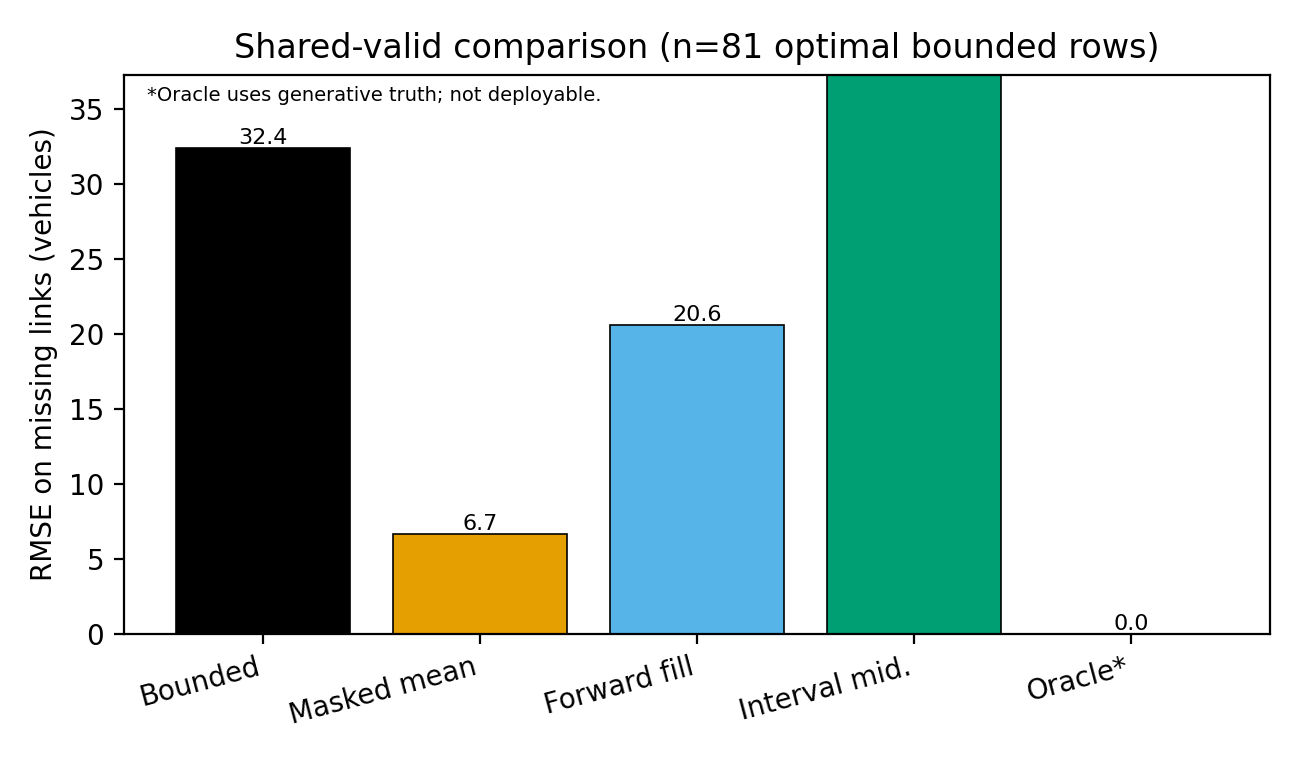
\includegraphics[width=0.92\linewidth]{figures/fig_primary_shared_valid.png}
  \caption{Shared-valid missing-link RMSE ($n=81$). Oracle bar uses generative truth and is not deployable.}
  \label{fig:primary}
\end{figure}

\begin{figure}[t]
  \centering
  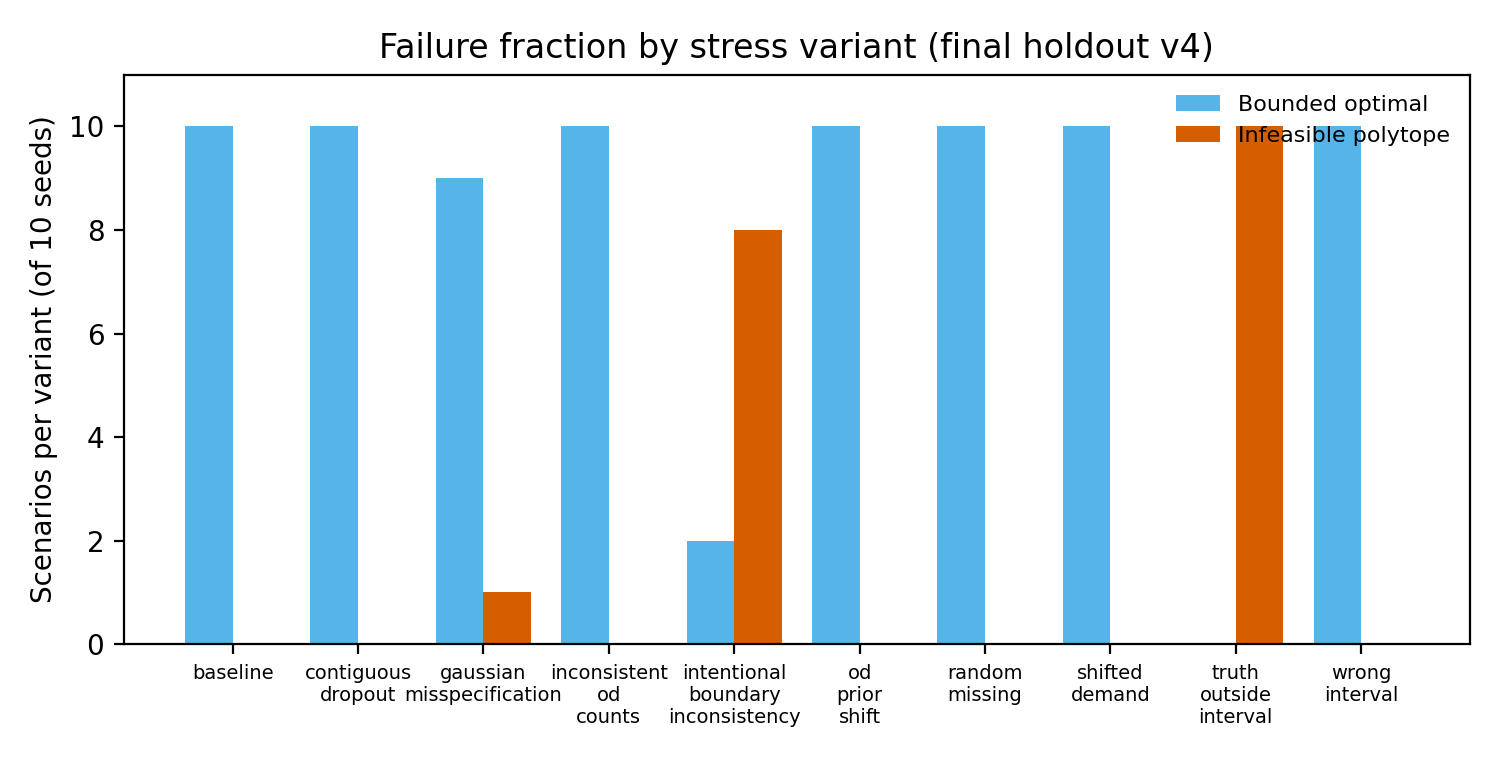
\includegraphics[width=0.92\linewidth]{figures/fig_infeasible_by_variant.png}
  \caption{Counts of optimal bounded solutions versus infeasible polytopes per stress variant (10 seeds each).}
  \label{fig:infeasible}
\end{figure}

\section{Illustrative non-identifiability (not a new theorem)}
When only a single aggregate of nonnegative path flows is observed with a wide upper bound, multiple
path splits remain feasible; the LP interval for total flow then has positive width even with perfect
count sensors on other links.
We include this as a textbook-style consequence of partial identification, not as a formal novelty claim.

\section{Discussion}
\textbf{Conservation versus accuracy.} Enforcing discrete balance and interval observations defines a
physically structured feasible set, yet on this synthetic holdout the deployable interior point does not
minimize missing-link RMSE relative to masked mean.

\textbf{Missing strong baselines.} Graph Markov networks~\cite{pu2020gmnn}, sparse Bayesian field estimators,
and physics-informed learning~\cite{shi2021pidl} are absent; any comparison would be speculative.

\textbf{Protocol amendments.} v4 followed a generative repair and failed v3 archive; it is not a blind repeat
of the original v3 preregistration.

\section{Limitations and future work}
Small chain geometry, a single completed final matrix, seed-cluster bootstrap with only ten clusters,
and no independent external OD truth limit external validity.
Fixing OD NNLS masking is documented but not applied to frozen v4.
Embargoed real-network adapters remain future work.

\section*{Declarations}
Author identity and contact appear on the title page.
See companion Markdown \texttt{AUTHOR\_VERIFICATION\_REQUIRED.md} for funding, ethics, and CRediT
attestations still requiring human confirmation.
AI assistance was used for manuscript packaging and literature verification; human authors remain
responsible for contributions and submission ethics.

\section*{Data and code availability}
Synthetic artifacts: \texttt{results/research\_final\_v4/}.
Table and figure regeneration:
\texttt{research\_manuscript/scripts/generate\_manuscript\_tables.py},
\texttt{make\_manuscript\_figures.py}.
Immutable input verification:
\texttt{research\_manuscript/scripts/verify\_immutable\_inputs.py}.
Layout: \texttt{arxiv.sty} from George Kour's MIT-licensed
\href{https://github.com/kourgeorge/arxiv-style}{arxiv-style} (see \texttt{TEMPLATE\_PROVENANCE.md}).

\bibliographystyle{plain}
\bibliography{references}

\end{document}
